\section{MIPS Assembly Implementation}
\subsection{Introduction}
\qquad In this project, we aim to emulate the Battleship game using the \textit{MIPS} assembly language. Due to resource constraints and to keep things simple, we will work with a smaller grid size which is \textbf{7$\times$7}
% \qquad A ship location is indicated by the
% coordinates of the bow and the stern of the ship (row$_{\text{bow}}$, column$_{\text{bow}}$, row$_{\text{stern}}$, column$_{\text{stern}}$).

\subsection{Overall Structure}
\begin{enumerate}
    \item \textbf{Data Section (.data):} \\
    The data section serves as the preamble to the program, laying the foundation for essential constants, character values, and game-related data. This section is crucial for establishing the groundwork necessary for the subsequent execution of the game.
        \begin{itemize}
            \item Constants: \\
            Various system calls are defined to facilitate operations such as \textit{printing} integers, strings, \textit{reading} integers, strings, and exiting. Additionally, character values are assigned to digits, letters, and spaces, enhancing the readability and manageability of the code.
            \item Game-related Constants: \\
            This subsection introduces constants that play a pivotal role in the game's mechanics. Values such as \textit{player turns}, the \textit{number of ships}, the \textit{number of cells}, and \textit{input lengths} are defined to ensure consistency and facilitate modifiability.
            \item Data and Variables: \\
            \textit{Arrays} for player A and player B maps are initialized, providing a structured representation of the game state. Strings containing the \textit{game title}, \textit{rules}, \textit{prompts}, and \textit{messages} are declared, contributing to a more comprehensible and user-friendly gaming experience.\\
            Numerous variables are introduced to store critical information, including the \textit{grid size}, \textit{ship coordinates}, and \textit{shot coordinates}. These variables serve as dynamic entities, adapting to the evolving state of the game during execution.
        \end{itemize}

    \item \textbf{Text Section (.text):} \\
    The text section constitutes the heart of the program, containing the main program logic, function calls, and the structural components that orchestrate the flow of the game. It encapsulates the core functionalities responsible for the game's initiation, progression, and termination.
        \begin{itemize}
            \item Main Section:\\
            The main section initializes registers, loads addresses for player maps, and orchestrates the initial setup of the game. It sets the stage for the subsequent execution of the game logic.
            \item Function Calls:\\
            Function calls to \texttt{game\_menu}, \textbf{rules\_screen}, and \texttt{print\_maps} contribute to the modular design of the code. These functions encapsulate specific functionalities, promoting code readability and maintainability.
            \item Game Setup:\\
            The code calls the \texttt{read\_ship} function twice, allowing players to input ship positions for player A and player B. After all the ships have been placed, the \texttt{print\_maps} function is invoked to visualize the current game state.
            \item Game Loop:\\
            The core game loop orchestrates the turn-based shooting mechanism, engaging players in strategic exchanges. Within the loop, players take turns calling the \texttt{read\_shot} function to input coordinates for targeting their opponent's fleet. After each successful shot, the program evaluates the game state to determine if the current player has won. If a player emerges victorious, the game loop concludes, and the \texttt{print\_maps} function is invoked to showcase the final game board with updated ship positions and the winner's triumph. This meticulous updating of the visual representation ensures that players are presented with a clear and conclusive view of the game's outcome.
            \item Exit Section:\\
            The program concludes with an \texttt{exit} section, invoking a system call to terminate the execution gracefully. This ensures proper closure and resource release.
        \end{itemize}

    \item \textbf{Helper Functions} \\
    This subsection delves into the specifics of key functions such as \texttt{read\_ship} and \texttt{read\_shot}. These functions are responsible for \textit{acquiring} user input, \textit{validating} it, and \textit{facilitating the corresponding game actions}.
\end{enumerate}


\subsection{Constants and Definitions}
Explain the purpose of constants defined using .eqv (e.g., system calls, characters, and game-related constants).

\begin{enumerate}
    \item \textbf{System Calls}:
    \begin{itemize}
        \item \texttt{SYS\_PRINT\_INT  \quad}: System call for printing an integer (value: 1).
        \item \texttt{SYS\_PRINT\_STRING}: System call for printing a string (value: 4).
        \item \texttt{SYS\_READ\_INT\qquad}: System call for reading an integer (value: 5).
        \item \texttt{SYS\_READ\_STRING }: System call for reading a string (value: 8).
        \item \texttt{SYS\_EXIT\qquad\qquad}: System call for program exit (value: 10).
        \item \texttt{SYS\_PRINT\_CHAR\quad}: System call for printing a character (value: 11).
        \item \texttt{SYS\_READ\_CHAR   \quad}: System call for reading a character (value: 12).
    \end{itemize}
    \item \textbf{Character Constants:} \\
    Constants representing ASCII values for characters:
    \begin{itemize}
        \item \texttt{char\_0} to \texttt{char\_6}: ASCII values for the characters '0' to '6'.
        \item \texttt{char\_N}: ASCII value for the character 'N'.
        \item \texttt{char\_Q}: ASCII value for the character 'Q'.
        \item \texttt{char\_R}: ASCII value for the character 'R'.
        \item \texttt{char\_Y}: ASCII value for the character 'Y'.
        \item \texttt{char\_n}: ASCII value for the character 'n'.
        \item \texttt{char\_q}: ASCII value for the character 'q'.
        \item \texttt{char\_r}: ASCII value for the character 'r'.
        \item \texttt{char\_y}: ASCII value for the character 'y'.
        \item \texttt{char\_space}: ASCII value for the space character.
    \end{itemize}
    \item \textbf{Player Turn and Game Constants:}
    \begin{itemize}
        \item \texttt{player\_a\_turn}: Value representing Player A's turn (value: 0).
        \item \texttt{player\_b\_turn}: Value representing Player B's turn (value: 1).
        \item \texttt{number\_of\_ships}: Total number of ships each player has (value: 6).
        \item \texttt{number\_of\_cells}: Total number of cells on the grid (value: 49).
        \item \texttt{input\_coordinates\_length\_shot}: Length of input for shot coordinates (value: 4).
        \item \texttt{input\_coordinates\_length\_ship}: Length of input for ship coordinates (value: 8).
    \end{itemize}
    \item \textbf{Player Maps and Grid Size:}
    \begin{itemize}
        \item \texttt{player\_a\_map}: An array representing the map for Player A, initialized with zeros.
        \item \texttt{player\_b\_map}: An array representing the map for Player B, also initialized with zeros.
        \item \texttt{grid\_size}: Word variable storing the size of the grid (value: 7).
    \end{itemize}   
    \item \textbf{Coordinate Spaces:}
    \begin{itemize}
        \item \texttt{ship\_coordinates}: Space reserved for storing ship coordinates during input.
        \item \texttt{shot\_coordinates}: Space reserved for storing shot coordinates during input.
    \end{itemize}
\end{enumerate}

These directives and data declarations provide symbolic names for system calls, characters, game constants, and storage spaces, making the MIPS assembly code more readable and maintainable. The constants and data structures defined here are used throughout the program to enhance code clarity and facilitate updates.\\

\newpage
\subsection{User Interface}
\begin{enumerate}
    \item \textbf{Game Menu:} \\
    
    The game menu is displayed to the user with ASCII art, creating a visually appealing and thematic presentation. The menu includes a title and options for the user to proceed or start the game. The ASCII art in the title creates a distinctive and engaging visual experience, making the menu more enjoyable for the user. The options to proceed or start the game are presented clearly to guide the user through the initial steps.\\

    \vspace*{2cm}

    \begin{figure}[H]
        \centering
        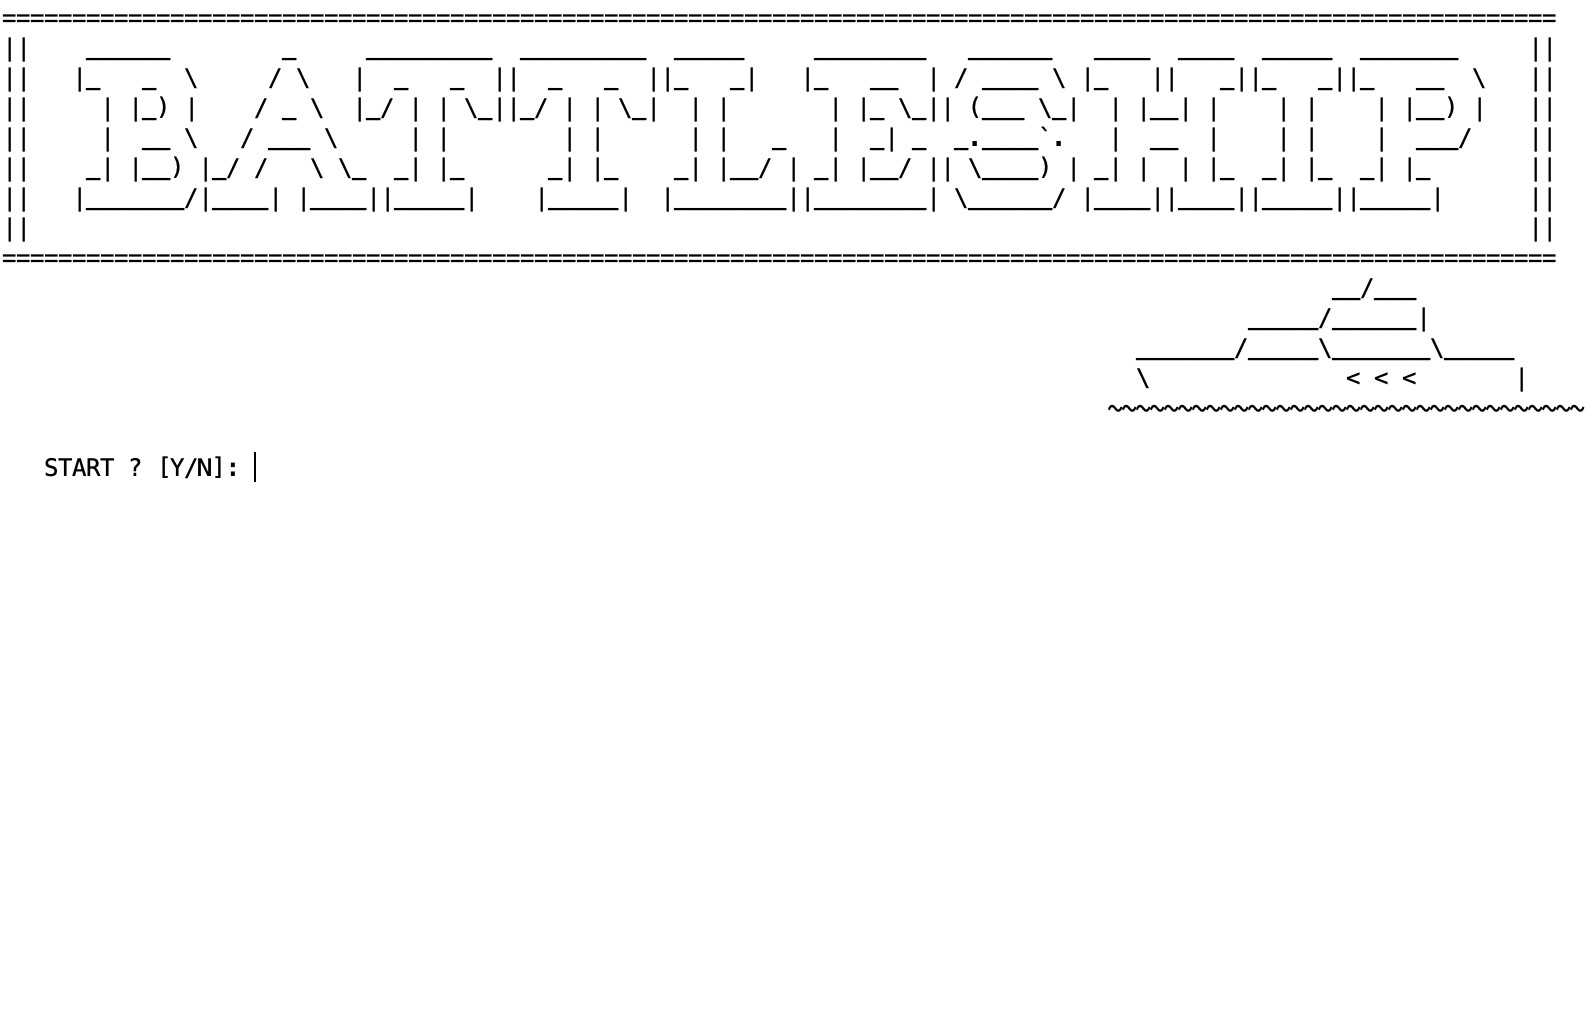
\includegraphics[width=15cm]{graphics/menu.jpg}
        \selectlanguage{english}
        \caption{Game Menu Interface}
    \end{figure}

    \newpage
    \item \textbf{Rules Screen:} \\
    
    The rules screen is presented using ASCII art to provide an immersive and visually interesting display of the game rules. The ASCII art includes a title, setup phase instructions, gameplay details, update board information, winning conditions, and specific rules about ship placement and shooting. Each section is delineated with ASCII borders and design elements, making it easy for the user to navigate and comprehend the rules of the game. The use of ASCII characters enhances the aesthetic appeal of the rules screen, making it both informative and visually engaging for the player.\\

    \begin{figure}[H]
        \centering
        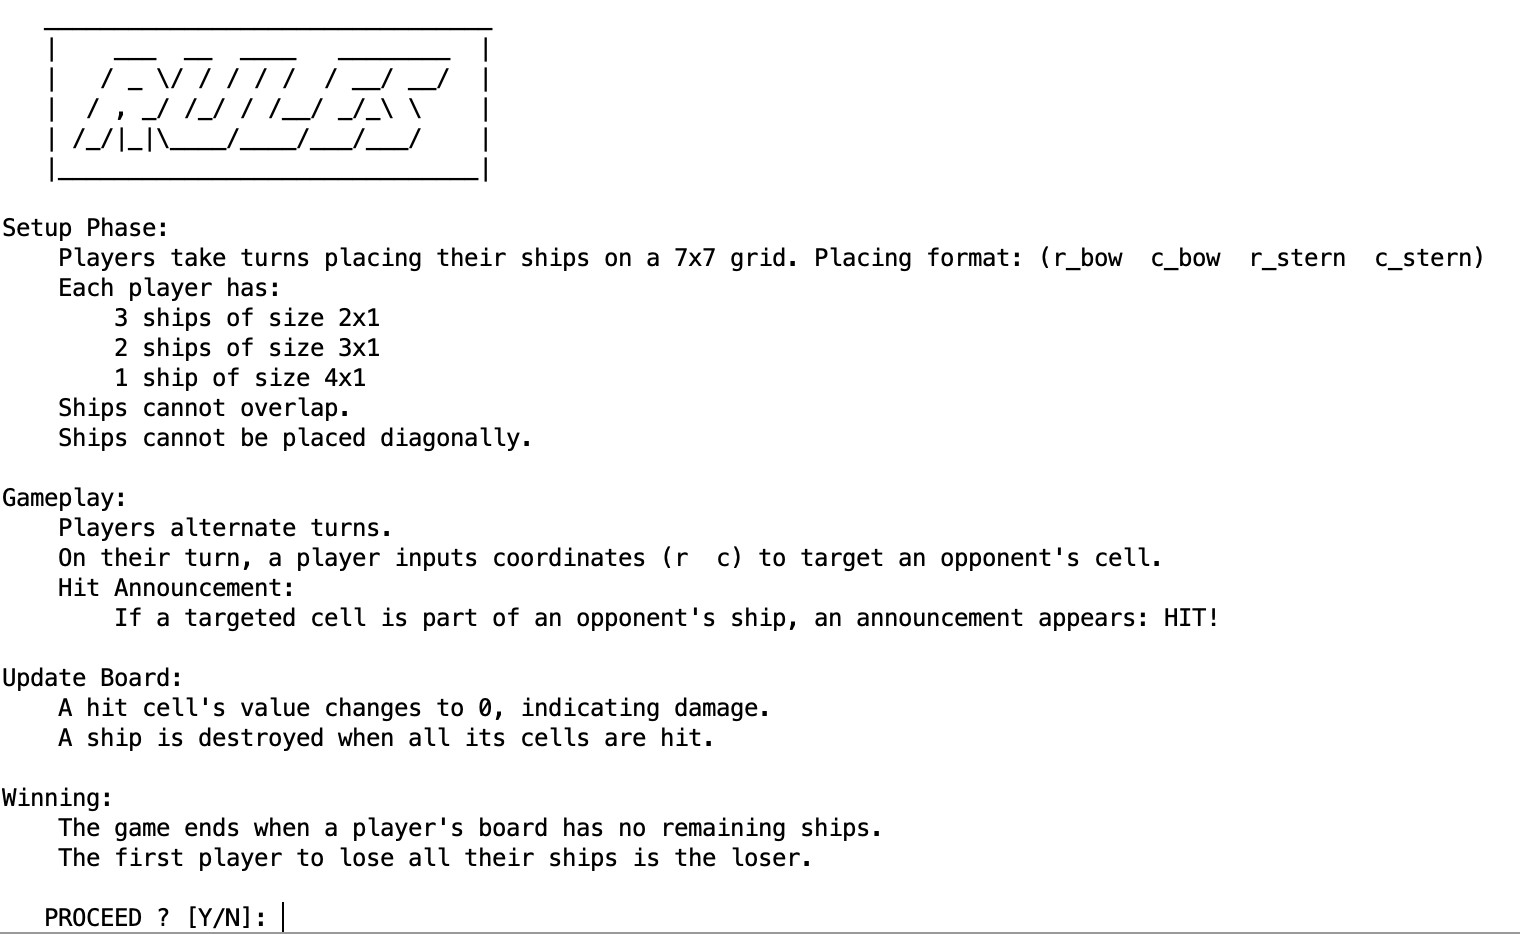
\includegraphics[width=15cm]{graphics/rules.jpg}
        \selectlanguage{english}
        \caption{Rules Screen Interface}
    \end{figure}

    \newpage
    \item \textbf{Initial Maps (For Grader):} \\
    
    In addition to the player-facing interface, there is a dedicated section for the grader to inspect the initial maps. These maps, represented as matrices, serve as the starting configuration for each player's game board. The matrix values denote ship placements and empty cells. This section aids the grader in evaluating the correctness of the initial game state, ensuring that the ships are appropriately positioned and adhere to the specified rules. The clarity of the ASCII art in the initial maps facilitates a quick and accurate assessment, streamlining the grading process.\\

    \begin{figure}[H]
        \centering
        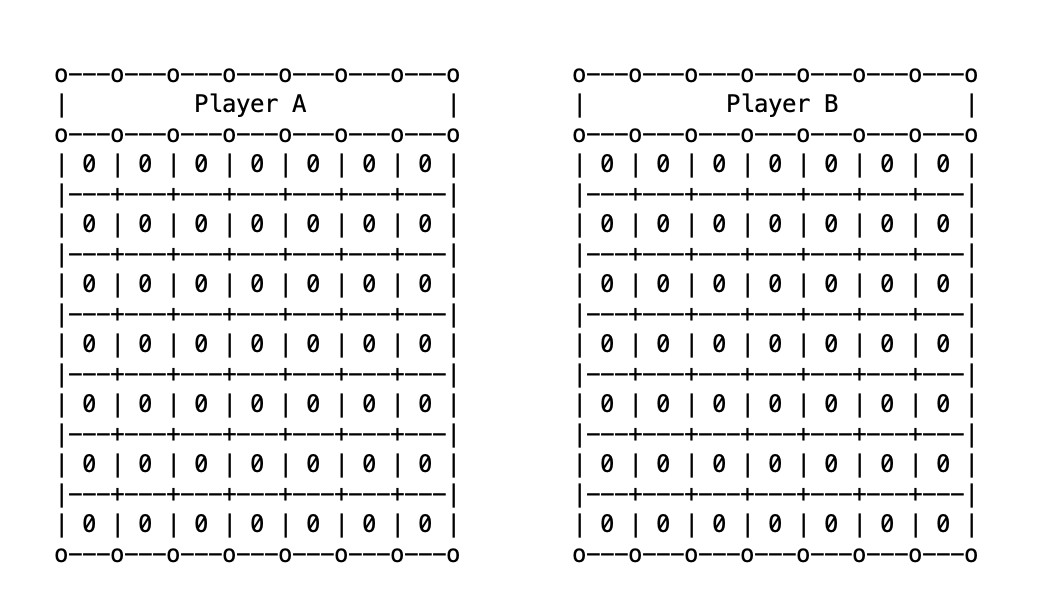
\includegraphics[width=15cm]{graphics/maps.jpg}
        \selectlanguage{english}
        \caption{Initial Maps Interface}
    \end{figure}
    
\end{enumerate}

\subsection{Game Logic}
Analyze the game flow from the main function.\\

Discuss how players take turns placing ships and shooting, including input validation.

\subsection{Helper Functions}
Describe the purpose of each function \(e.g., game_menu, rules_screen, read_ship, read_shot\).\\

Highlight the functionality of key functions and their interaction.

\subsection{Input Validation - Error Handling}
Discuss how the code validates user input for ship and shot coordinates. \\

Analyze the error messages and how they guide the user.

\subsection{Gameplay Logic}
Explain the sequence of events during ship placement and shooting.\\

Discuss how ships are drawn on the maps and the conditions for hitting or missing.